%--------------- Personalize your document here ---------------

\author{
\\ Djan Tanova 2542341t} % Enter your name

\newcommand{\studentID}{} % enter your Team No
\newcommand{\department}{School ofEngineering}
\newcommand{\course}{Quantum ELectronic Devices}

\title{Lab 1} %Enter the title of your report 
\date{February 2024} % insert a specific date	

% \newcommand{\supervisorone}{Supervisor 1} % Enter your supervisor's name
% \newcommand{\supervisortwo}{Supervisor 2}% Leave it empty or enter your second supervisor's name 
%--------------------------------------------------------------



\documentclass[a4paper,12pt]{article}
\usepackage[left=30mm,top=30mm,right=30mm,bottom=30mm]{geometry}
\usepackage{etoolbox} %required for cover page
\usepackage{booktabs}
\usepackage[usestackEOL]{stackengine}
\usepackage[T1]{fontenc}
\usepackage[utf8]{inputenc}
\usepackage{bm}
\usepackage{svg}
\usepackage{graphicx}
\usepackage{subcaption}
\usepackage{amsmath}
\usepackage{amsfonts}
\usepackage{mathtools}
\usepackage{xcolor}
\usepackage{float}
\usepackage{hyperref}
\usepackage[capitalise]{cleveref}
\usepackage{enumitem,kantlipsum}
\usepackage{amssymb}
\usepackage[square,numbers,sort]{natbib}
\usepackage[ruled,vlined]{algorithm2e}
\usepackage{listings}
\usepackage{minted}
\usemintedstyle{emacs}

\renewcommand{\listingscaption}{Algorithm}
\renewcommand{\listoflistingscaption}{List of Algorithms}

%noindent
\setlength\parindent{0pt}

\bibliographystyle{unsrtnat}

\hypersetup{
    colorlinks,
    linkcolor={black},
    citecolor={blue!50!black},
    urlcolor={blue!80!black}
}

\definecolor{codegreen}{rgb}{0,0.6,0}
\definecolor{codegray}{rgb}{0.5,0.5,0.5}
\definecolor{codepurple}{rgb}{0.58,0,0.82}
\definecolor{backcolour}{rgb}{0.95,0.95,0.92}

\lstdefinestyle{mystyle}{
    backgroundcolor=\color{backcolour},   
    commentstyle=\color{codegreen},
    keywordstyle=\color{magenta},
    numberstyle=\tiny\color{codegray},
    stringstyle=\color{codepurple},
    basicstyle=\ttfamily\footnotesize,
    breakatwhitespace=false,         
    breaklines=true,                 
    captionpos=b,                    
    keepspaces=true,                 
    numbers=left,                    
    numbersep=5pt,                  
    showspaces=false,                
    showstringspaces=false,
    showtabs=false,                  
    tabsize=2
}

\lstset{style=mystyle}

\linespread{1}

\newtheorem{theorem}{Theorem}[section]
\graphicspath{{figures/}}	

%----------------------------------TITLE PAGE -----------------------------------
\makeatletter
\def\maketitle{
  \begin{center}\leavevmode
       \normalfont
       
\includegraphics[width=1\columnwidth]{UoG Logo Transparent BG.png}
       \vskip 1.5cm   
       \textsc{\large \department}\\
       \vskip 1.5cm
       \rule{\linewidth}{0.3 mm} \\
       \vskip 0.5cm
       {\large \course}\\[1 cm]
       {\huge \bfseries \@title \par}
       \vspace{0.7cm}
	\rule{\linewidth}{0.2 mm} \\[1.5 cm]
	
    \textbf{\large \@author}
	\vskip 0.5cm
	\textbf{\studentID}	
	

	\vfill
	{\Large \@date\par}
   \end{center}
   %\vfill
   %\null
   \cleardoublepage
  }
\makeatother


%-------------------------------- ENDTITLE PAGE ----------------------------------

\begin{document}

\pagenumbering{gobble}% Remove page numbers (and reset to 1)

\maketitle

\clearpage
\tableofcontents
\clearpage


\pagenumbering{arabic}% Arabic page numbers (and reset to 1)

% This is how you can organize your document
\section{Task 1: Energy Eigenvalues }
\subsection{Calculating the Eigenvalues}
In this task we were asked to calculate eigenvalues for a wave function in a well for quantum numbers up to \(n = 5\). The following code achieves that function.

\begin{lstlisting}[language=Python, caption= Code used to obtain E_n values]
    from scipy import constants

h_bar = constants.hbar
e_mass = constants.m_e
a = 1 * 10e-10

def get_eigenvalue(q_number: int, a = 1 * 10e-10):
    E_n = pow(constants.pi * h_bar * q_number, 2) / (2*e_mass* pow(a,2)) 
    return E_n


n_vals = np.linspace(1,5,5, dtype=int)
E_n = []
E_1 = get_eigenvalue(1)

# Increase figure size
plt.figure(figsize=(6, 6))
x_list = np.linspace(0.01, 10, 20)
for n in n_vals:
    E_new = get_eigenvalue(n)
    E_n.append(E_new)
    
    if (E_new == pow(n,2)*E_1):
        print("eqn is right! n:", n)
    else:
        print("eqn is wrong! n:", n)

    plt.plot(x_list, plotty(E_new), linewidth=2)



# Set thicker frame
plt.gca().spines['top'].set_linewidth(1.25)
plt.gca().spines['right'].set_linewidth(1.25)
plt.gca().spines['bottom'].set_linewidth(1.25)
plt.gca().spines['left'].set_linewidth(1.25)

# Set larger tick marks pointing in
plt.tick_params(axis='both', which='both', direction='in', width=1.25, size = 6)

# Set larger tick labels
plt.xticks(fontsize=16)
plt.yticks(fontsize=16)

# Add legend with larger font
plt.legend(["n = " + str(n) for n in n_vals], bbox_to_anchor=(1.05, 1.0), loc='upper left', fontsize=16)

# Set larger axis labels
plt.xlabel("$x_{list}$ (units)", fontsize=18)
plt.ylabel("$E$ (J)", fontsize=18)

# Save and show plot
plt.savefig('E_n.png', bbox_inches='tight')
plt.show()
\end{lstlisting}

The code generates the following graph. The graph accurately depicts the expected \(E_n\) values with the relationship \(E_n = n^2 * E_1 \).
\begin{figure}[H]          
    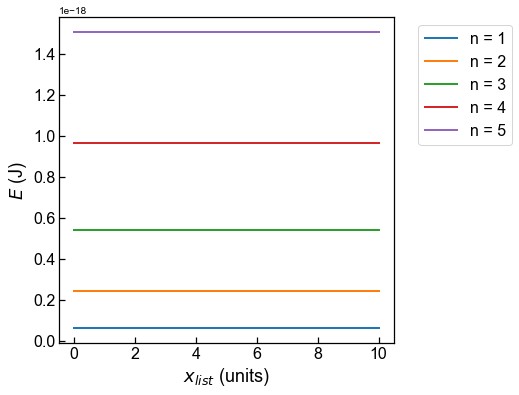
\includegraphics[width=\columnwidth]{report/figures/E_n.png}
    \caption{Energy eigenvalues, \(E_n\), for varying quantum numbers. }
    \label{fig:enter-label}
\end{figure}

\section{Task 2: Eigenfunctions}
\subsection{Calculating Eigenfunctions}
For this task we were asked to plot a depiction of the normalised wavefunctions, i.e. eigenfunctions, for the given wave function, with the quantum number up to \(n=3\). 

\begin{lstlisting}[language=Python, caption= Code used to plot findings]
def psi_n(q_number, x_values, a = 1 * 10e-10):
    """
    Creates a list of corresponding y values given a list of x values.
    """
    A_n = np.sqrt(2/a)
    k_n = (q_number*np.pi)/a
    return A_n * np.sin(k_n*x_values)

x_list = np.linspace(0, a, 50)
# Increase figure size
plt.figure(figsize=(10, 10))

n_vals = np.linspace(1,3,3)
for n in n_vals:
    plt.plot(x_list, psi_n(n, x_list), linewidth=2)

# Set thicker frame
plt.gca().spines['top'].set_linewidth(1.25)
plt.gca().spines['right'].set_linewidth(1.25)
plt.gca().spines['bottom'].set_linewidth(1.25)
plt.gca().spines['left'].set_linewidth(1.25)

# Set larger tick marks pointing in
plt.tick_params(axis='both', which='both', direction='in', width=1.25, size = 6)

# Set larger tick labels
plt.xticks(fontsize=16)
plt.yticks(fontsize=16)

# Add legend with larger font
plt.legend(["n = " + str(n) for n in n_vals], bbox_to_anchor=(1.05, 1.0), loc='upper left', fontsize=16)

# Set larger axis labels
plt.xlabel("$Well Length$ (m)", fontsize=18)
plt.ylabel("$psi_n$", fontsize=18)

# Save and show plot
plt.savefig('psi_n.png', bbox_inches='tight')
\end{lstlisting}

\subsubsection{Analysis of Graph Generated}
\begin{figure}[H]
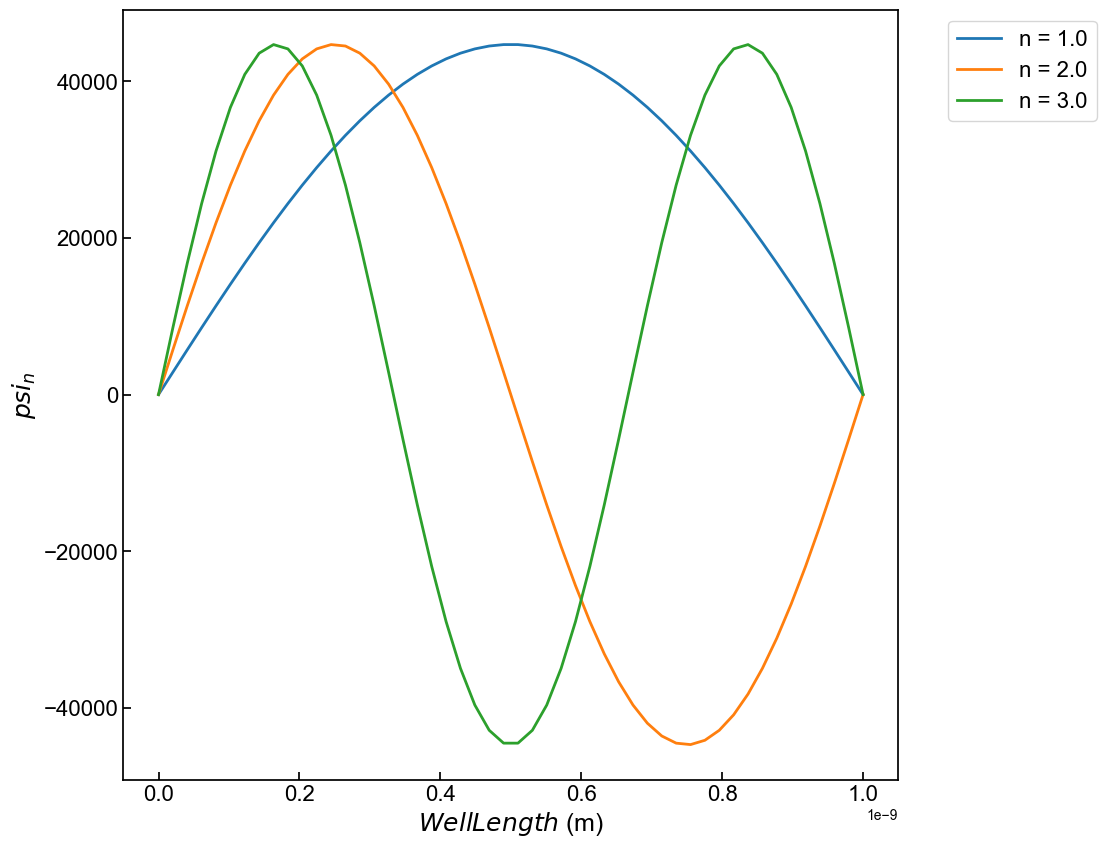
\includegraphics[width=\columnwidth]{report/figures/psi_n.png}
\caption{Plots of eigenfunctions}
\end{figure}
From the figure, we can see that the behaviour of the wavefunction in the well. The frequency of the wave is proportional to the quantum number, which is as expected. 

\subsection{Calculating Probability Density}
\subsubsection{Calculating P_n}
For the given wave functions, we then calculated the probability density functions, \(P_n = |\Psi_n(x)|^2\).

\begin{lstlisting}[language=Python, caption= Code used to plot findings]
x_list = np.linspace(0, a, 100)
# Increase figure size
plt.figure(figsize=(10, 10))

n_vals = np.linspace(1,3,3)
for n in n_vals:
    plt.plot(x_list, np.power(np.abs(psi_n(n, x_list)),2), linewidth=2)

# Set thicker frame
plt.gca().spines['top'].set_linewidth(1.25)
plt.gca().spines['right'].set_linewidth(1.25)
plt.gca().spines['bottom'].set_linewidth(1.25)
plt.gca().spines['left'].set_linewidth(1.25)

# Set larger tick marks pointing in
plt.tick_params(axis='both', which='both', direction='in', width=1.25, size = 6)

# Set larger tick labels
plt.xticks(fontsize=16)
plt.yticks(fontsize=16)

# Add legend with larger font
plt.legend(["n = " + str(n) for n in n_vals], bbox_to_anchor=(1.05, 1.0), loc='upper left', fontsize=16)

# Set larger axis labels
plt.xlabel("$Location$ (m)", fontsize=18)
plt.ylabel("$P_n$", fontsize=18)

# Save and show plot
plt.savefig('P_n.png', bbox_inches='tight')
\end{lstlisting}

\subsubsection{Analysis of Graph Generated}
\begin{figure}[H]
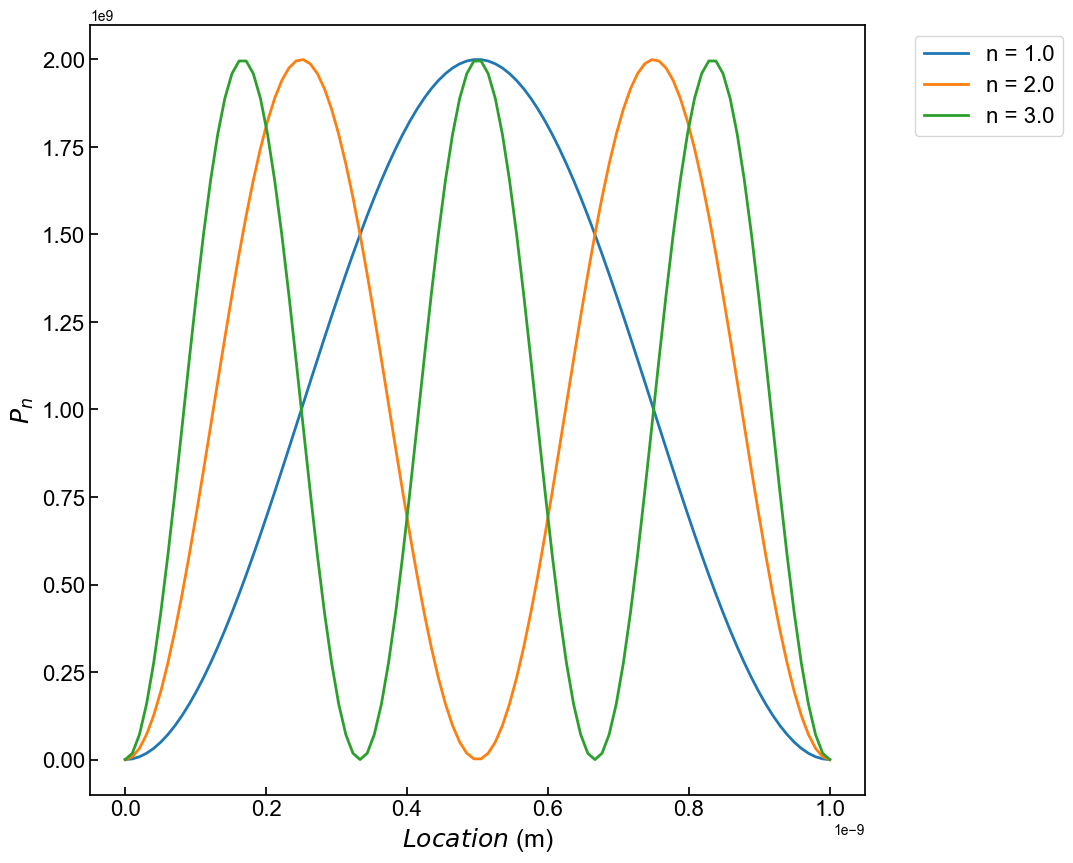
\includegraphics[width=\columnwidth]{report/figures/P_n.png}
\caption{Plots of P_n, n=1,2,3}
\end{figure}
From the figure, we can see the probability density of the wavefunctions in the well. The number of peaks in probability is proportional to the quantum number, which is as expected. 

\section{Task 3: Superposition}
\subsubsection{Calculating \(\Psi(x,t)\)}
For the given wave functions, \(\psi_n\) and \(\psi_m\) we used the following code to calculate the resulting superposition wave function, \(\Psi(x,t)\).

\begin{lstlisting}[language=Python, caption= Code used to plot findings]
from matplotlib.animation import FuncAnimation

def psi_m(q_number, x_values, a = 1.1 * 10e-10):
    """
    Creates a list of corresponding y values given a list of x values.
    """
    A_n = np.sqrt(2/a)
    k_n = (q_number*np.pi)/a
    return A_n * np.sin(k_n*x_values)

def Psi_s(psi_n, psi_m, q_number: int, x_values: list, t_values: list):
    A_n = A_m = 1 #Assume amplitudes of both waves are 1
    E_n = get_eigenvalue(q_number+1)
    E_m = get_eigenvalue(q_number, a= 1.1 * 10e-10) # Assume both wavefunctions have the same quantum number
    Psi_s_t = [A_n*psi_n(q_number,x_values)*np.float_power(np.e, (-1j * E_n * t / constants.hbar )) + A_m*psi_m(q_number,x_values)*np.float_power(np.e, (-1j * E_m * t / constants.hbar )) for t in t_values]
    return Psi_s_t

num_frames = 1000
x_list = np.linspace(0, 1.1 * 10e-10, 500)
t_list = np.linspace(0, 1, num_frames)
Psi = Psi_s(psi_n, psi_m, q_number=2, x_values= x_list, t_values= t_list)

plt.figure(1)

fig, (ax1,ax2, ax3) = plt.subplots(1,3)
ax1.plot( x_list, np.real(Psi[0]))
ax1.set_title("t = "+ str(t_list[0]) )
ax2.plot( x_list, np.real(Psi[num_frames//2]))
ax2.set_title("t = "+str(t_list[num_frames//2]))
ax3.plot( x_list, np.real(Psi[int(num_frames*0.9)]))
ax3.set_title( "t = "+str(t_list[int(num_frames*0.9)]))
ax1.sharey(ax2)
ax3.sharey(ax2)

fig.suptitle("Time Evolution of Superposition")
plt.savefig('super_steps.png', bbox_inches='tight')
plt.figure(2)
# Create a figure and axis
fig, ax = plt.subplots()
line, = ax.plot(x_list, np.real(Psi[0]), label="Re(Psi_s)")

# Set axis limits
ax.set_xlim(0, a)

# Add labels and title
ax.set_xlabel("Position (m)")
ax.set_ylabel("Wavefunction")
ax.set_title("Time Evolution of Superposition")

# Animation update function
def update(frame):
    line.set_ydata(np.real(Psi[frame]))
    return line,

# Create the animation
ani = FuncAnimation(fig, update, frames=len(t_list), interval=200, blit=True)

# Save the animation (optional)
ani.save("wavefunction_animation.gif", writer="ffmpeg")

# Show the animation
plt.show()

\end{lstlisting}

\subsubsection{Analysis of Graph Generated}
\begin{figure}[H]
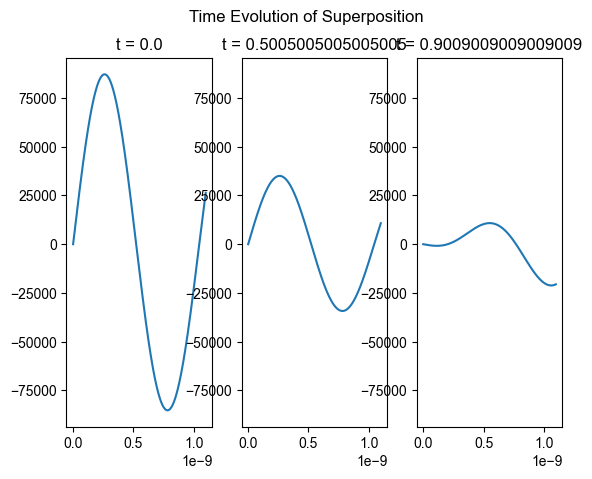
\includegraphics[width=\columnwidth]{report/figures/super_steps.png}
\caption{Plots of \(\Psi(x,t)\) at different t values}
\end{figure}
From the figure, we can see the product of the superimposed wavefunctions in the well at different points in time. Due to superposition, we would expect a time dependent product of two non time dependent wave functions. The resulting plot accurately represents this. 
\clearpage

\end{document}